
\section{Figures}

\begin{figure}[h]
        \begin{center}
        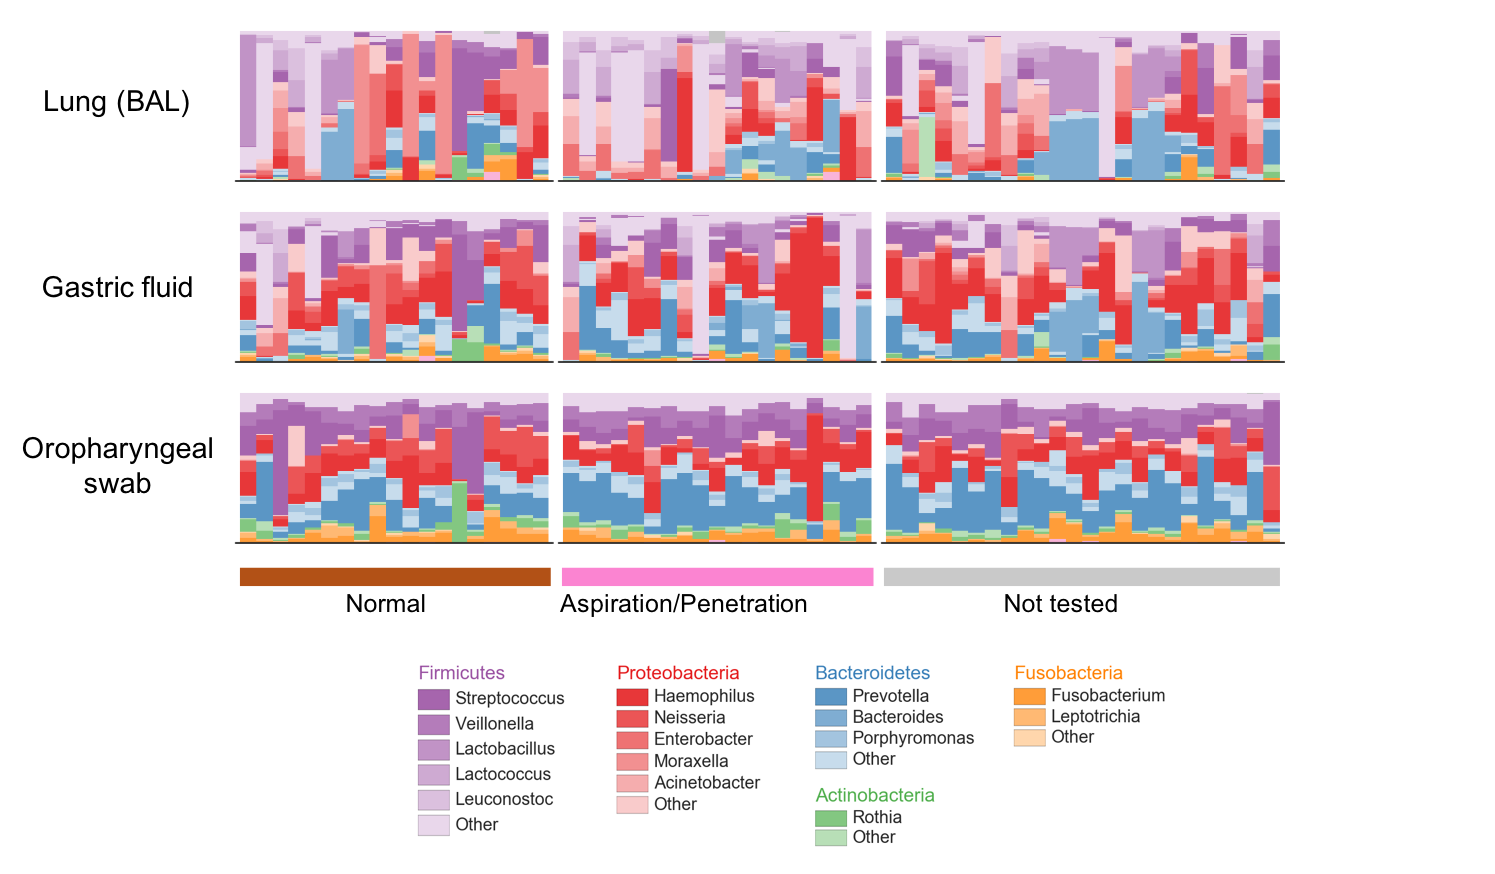
\includegraphics[width=1.2\textwidth]{community_overview_whitebckg.png}
        \caption{\textbf{Aerodigestive communities have similar predominant genera.} Bar plots showing relative abundances of aerodigestive OTUs collapsed to the genus level. Each column corresponds to one patient who had all three aerodigestive sites sequenced (N $=$ 19 non-aspirators, 23 aspirators, 24 untested). Phyla in legend are those with mean abundance $>$ 0.01 across all patients. Any other phyla are colored gray.}
        \label{fig:overview_plots}
        \end{center}
\end{figure}

\begin{figure}[h]
        \begin{center}
        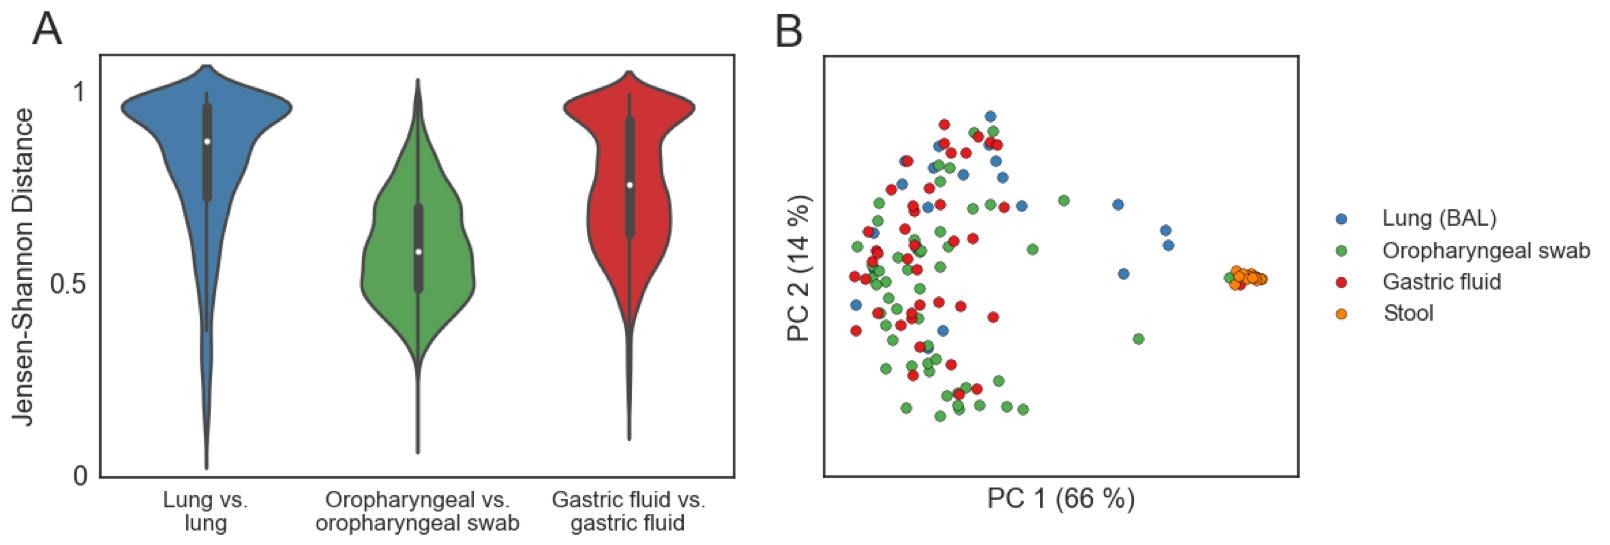
\includegraphics[width=\textwidth]{baseline_aerodigestive_across_patients_whitebckg.png}
        \caption{\textbf{Lung and gastric communities are more variable across people than oropharyngeal communities.} (A) Violin plot of the Jensen-Shannon distance (JSD) between samples from the same site across different patients. A JSD close to 1 indicates that communities are very different (less similar). (B) PCoA plots of aerodigestive and stool microbial communities for all patients in the 2016 sequencing batch (N $=$ 21 BAL, 52 oropharyngeal swab, 43 gastric fluid, and 14 stool samples).}
        \label{fig:across_people}
        \end{center}
\end{figure}

\begin{figure}[h]
        \begin{center}
        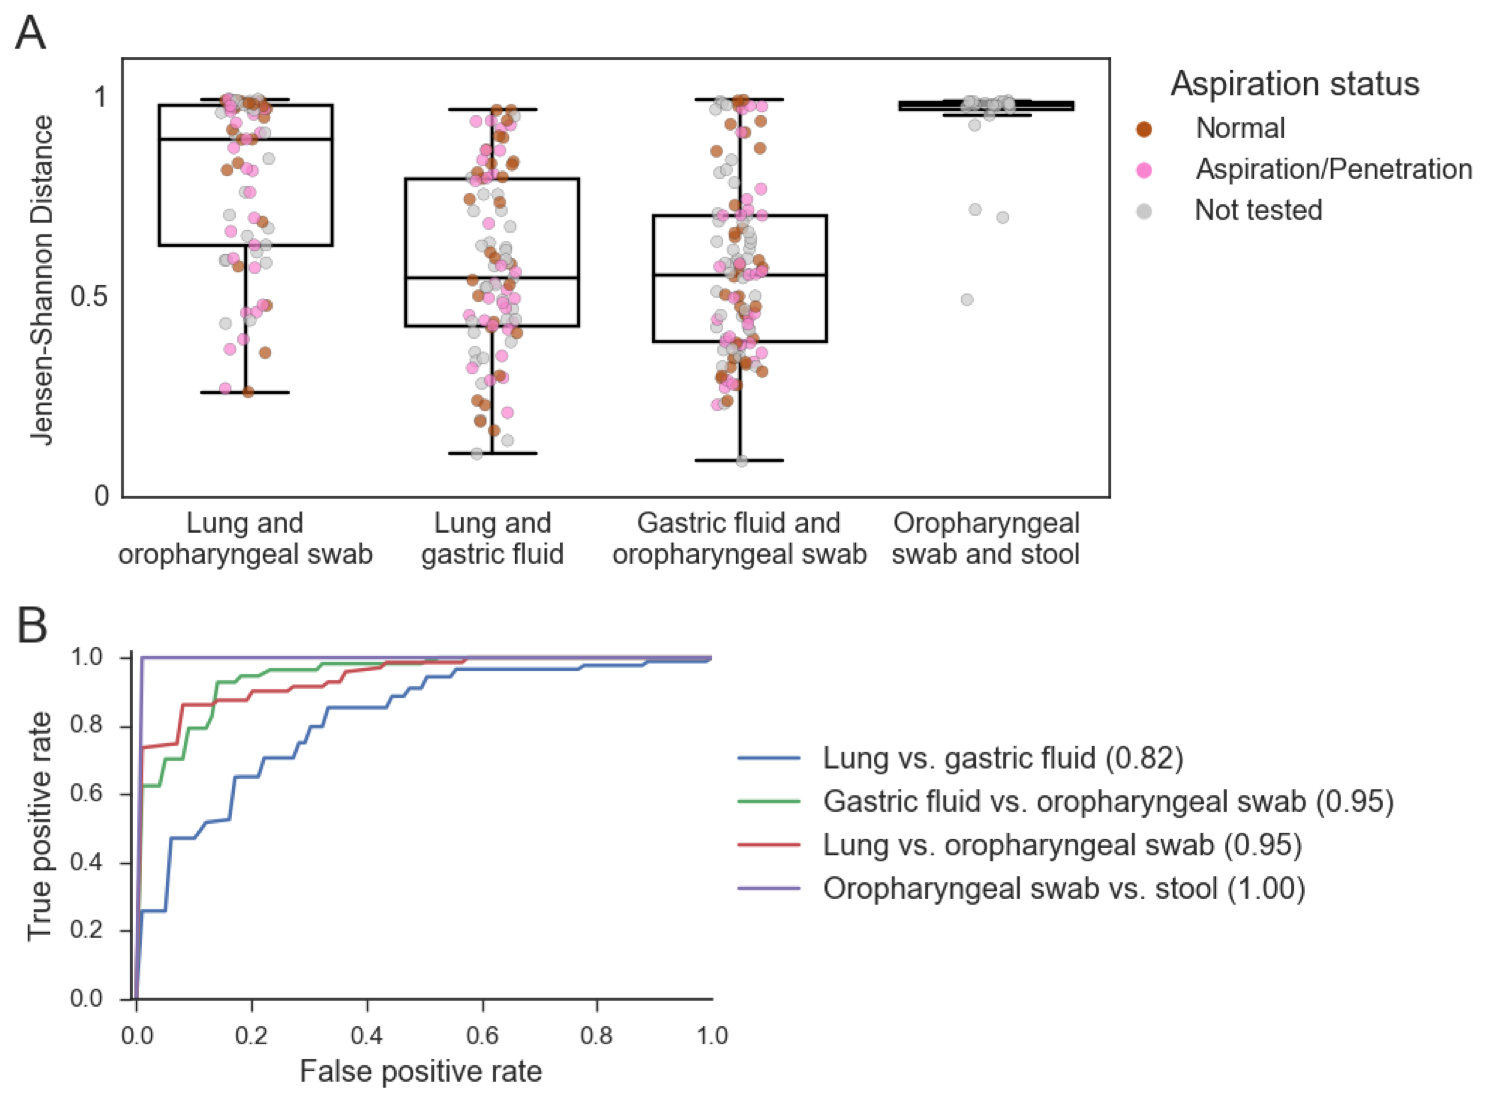
\includegraphics[width=\textwidth]{baseline_aerodigestive_within_patients_whitebckg.png}
        \caption{\textbf{Within patients, aerodigestive communities are similar but lung and oropharynx remain most distinct.} (A) Jensen-Shannon distances between samples from different sites from the same patient. Comparisons between stool and oropharynx are included to contextualize these results, as these are expected to be very different. All comparisons are significant (Wilcoxon rank sums test calculated with Python's \texttt{scipy.stats.ranksums} function) except the lung and gastric fluid vs. gastric fluid and oropharyngeal swab beta diversities (p $=$ 0.6). Lung and oropharyngeal vs. oropharyngeal and stool, p $=$ 0.005. All other comparisons:  $p < 1 \times 10^{-8}$. (B) ROC curve of classifiers distinguishing different aerodigestive sites. Mean areas under the ROC curve (AUCs) are reported in parentheses in the legend.}
        \label{fig:within_patients}
        \end{center}
\end{figure}

\begin{figure}[h]
        \begin{center}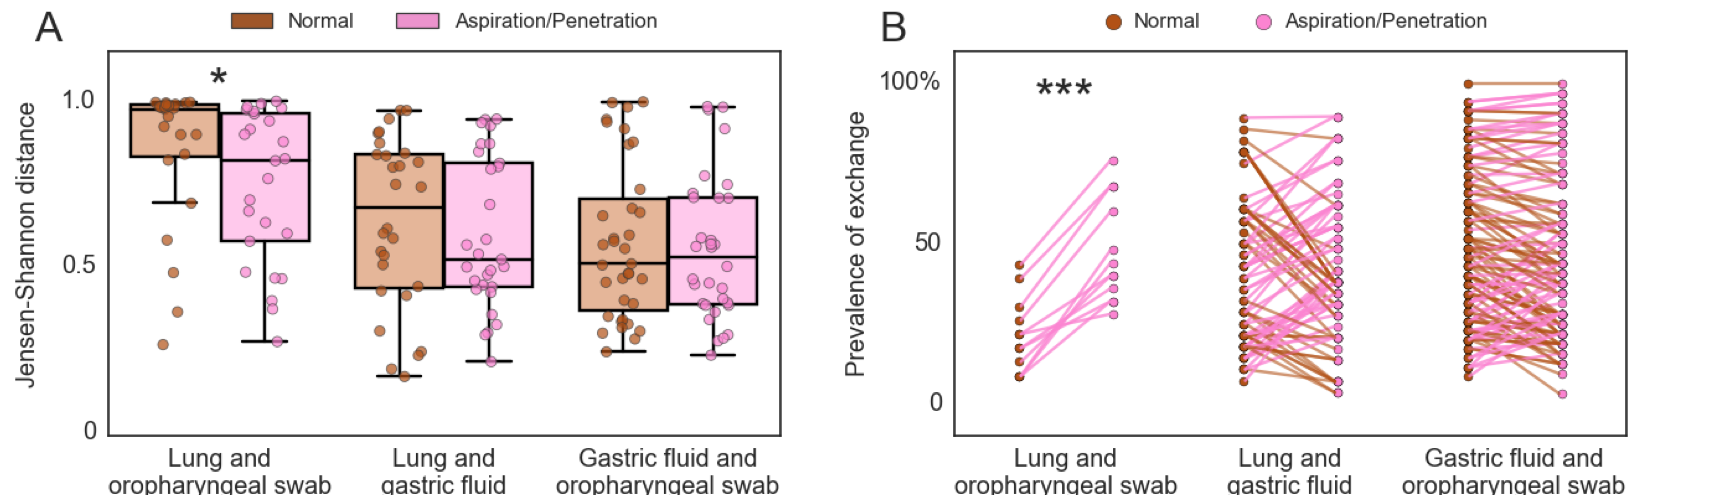
\includegraphics[width=\textwidth]{aspiration_jsd_exchange_whitebckg.png}
        \caption{\textbf{Dysphagia increases aspiration of microbes from the oropharynx but not the stomach} (A) Intra-patient Jensen Shannon distance for different aerodigestive site comparisons in non-aspirators (brown) and aspirators (pink). Each point represents one patient. P-values (Wilcoxon rank sums test, calculated with Python's \texttt{scipy.stats.ranksums} function): lung and oropharyngeal swab $p = 0.04$, lung and gastric fluid $p = 0.5$, gastric fluid and oropharyngeal swab $p = 0.8$. (B) Percentage of patients with the previously defined exchanged microbes present in both of the respective sites (x-axis) in non-aspirators (brown) and aspirators (pink). Each pair of points represents one exchanged OTU. P-values (paired t-test on $log_{10}$ prevalence values, calculated with Python's \texttt{scipy.stats.ttest\_rel} function: lung and oropharyngeal swab $p = 3 \times 10^{-5}$, lung and gastric fluid $p = 0.8$, gastric fluid and oropharyngeal swab $p = 0.09$.}
        \label{fig:aspiration}
        \end{center}
\end{figure}

\begin{figure}[h]
        \begin{center}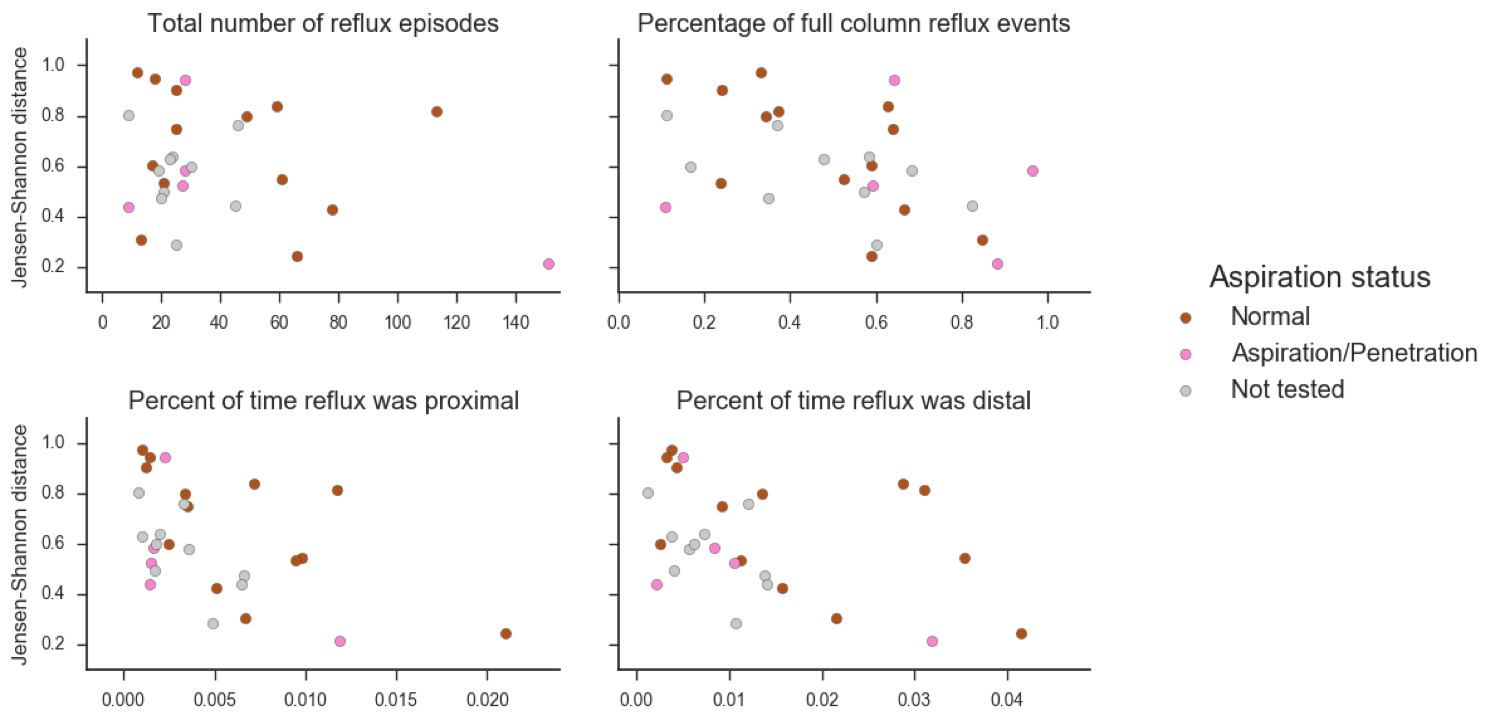
\includegraphics[width=\textwidth]{reflux_correlation_with_bal_gastric.png}
        \caption{\textbf{Reflux severity may correlate with the similarity between lung and gastric communities.} Each plot shows the correlation between different reflux measures and the within-patient Jensen-Shannon distance between BAL and gastric fluid samples. Points are colored according to aspiration status. All reflux measures include both acid- and non-acid reflux. Spearman correlation and p-values: total number of reflux episodes $\rho_s = -0.14, p = 0.5$, percentage of full column reflux events $\rho_s = -0.41, p = 0.03$, percent of time reflux was proximal $\rho_s = -0.47, p = 0.01$, percent of time reflux was distal $\rho_s = -0.43, p = 0.02$.}
        \label{fig:reflux_corr}
        \end{center}
\end{figure}
